\documentclass[11pt,oneside,openright]{memoir}

\usepackage{tcolorbox}
\usepackage[scaled]{beramono}
\renewcommand*\familydefault{\ttdefault}
\usepackage[T1]{fontenc}
\usepackage{tabularx}
\usepackage{listings}
\usepackage{graphicx}
\usepackage{xcolor}
\usepackage{tikz}
\usepackage{pgfplots}
\usepackage{pgfplotstable}

\pgfplotstableread[col sep=comma]{
start,end,Name,color
0,600000,fooer,color1
600000,1020000,foo2bar,color2
}\loadedtable

\definecolor{color1}{RGB}{146,200,180}
\definecolor{color2}{RGB}{124,206,89}

\begin{document}
\pagestyle{plain}
\noindent
\begin{minipage}{\textwidth}
    \vspace{-8em}\hspace{-8em}
    
\includegraphics[width=9em]{images/scipipe_logo_bluegrey.pdf}
\end{minipage}

\noindent 
{\huge\textbf{SciPipe workflow report}}
\vspace{10pt}

    \begin{tcolorbox}[ title=My workflow, ]
    \small
\begin{tabular}{rp{0.72\linewidth}}
SciPipe version: & 0.7 \\
Start time:  & 2018-06-28 8:40:00.000000000 +0200 CEST \\
Finish time: & 2018-06-28 8:50:00.000000000 +0200 CEST \\
Run time: &   \\
\end{tabular}
    \end{tcolorbox}

\vfill

\setlength{\fboxsep}{0pt}
\noindent
\hspace{-0.1725\textwidth}\fbox{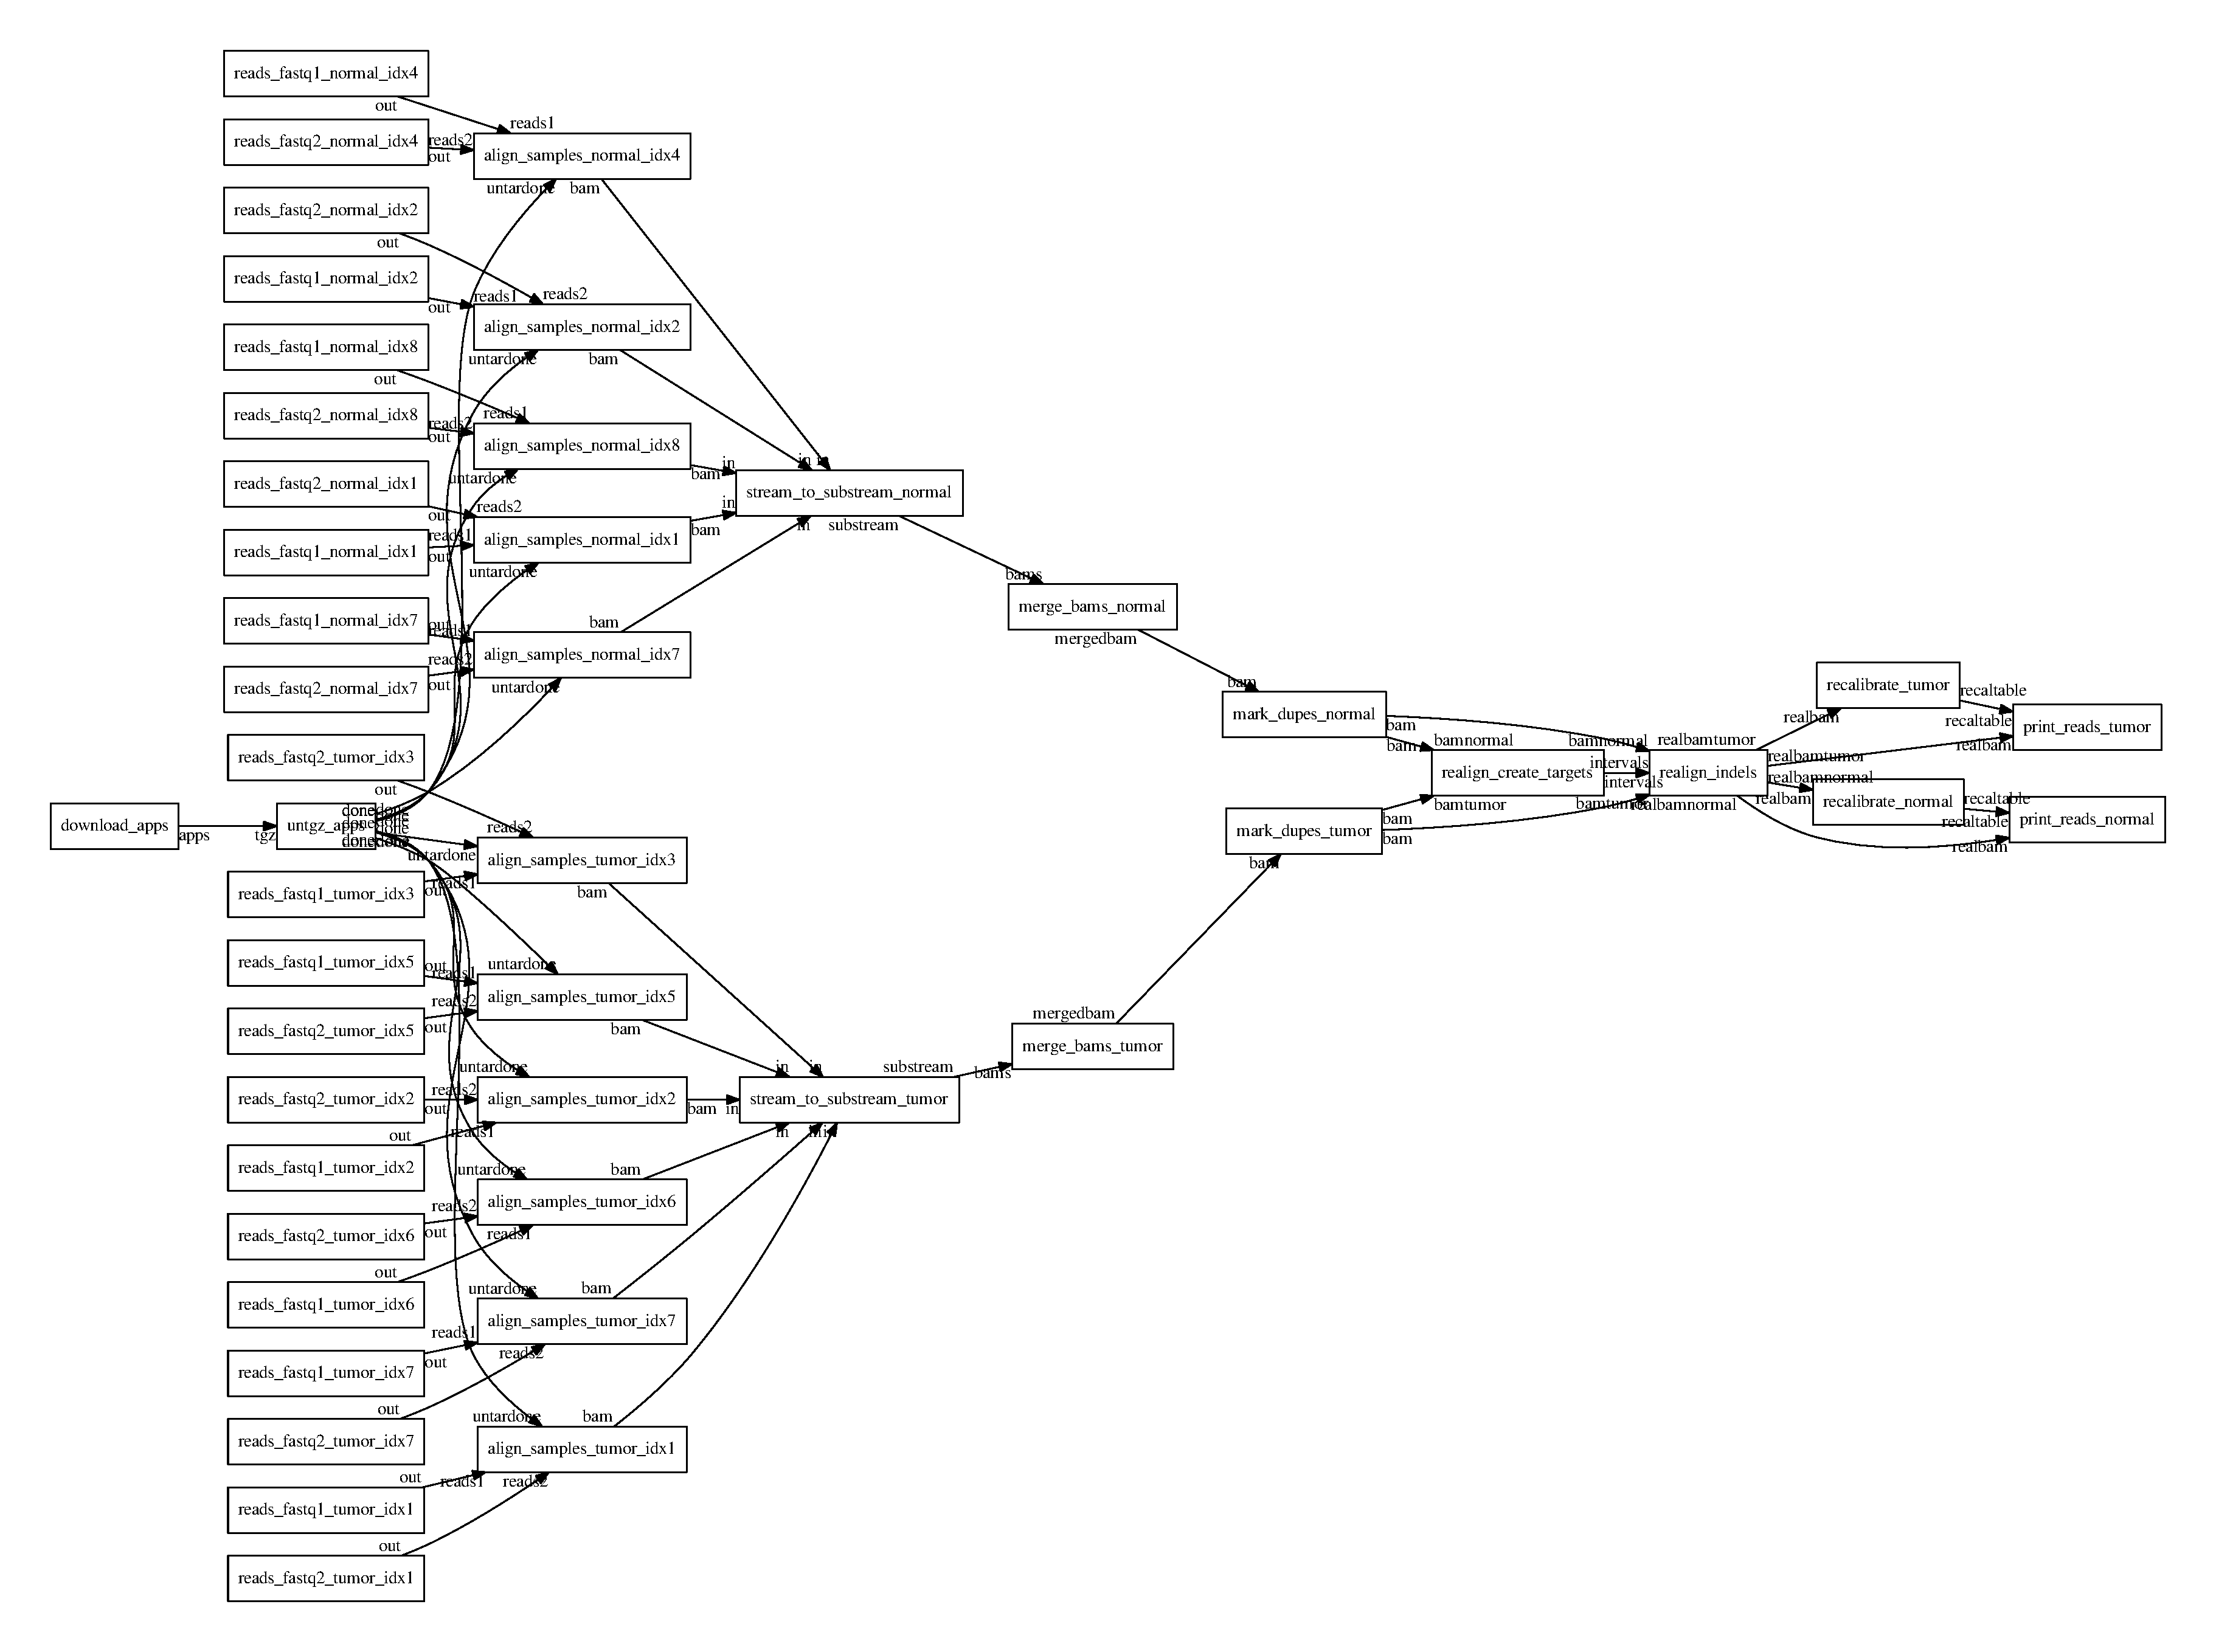
\includegraphics[width=1.35\textwidth]{cawpre.pdf}}
\vfill
\newpage

\section*{Execution timeline}

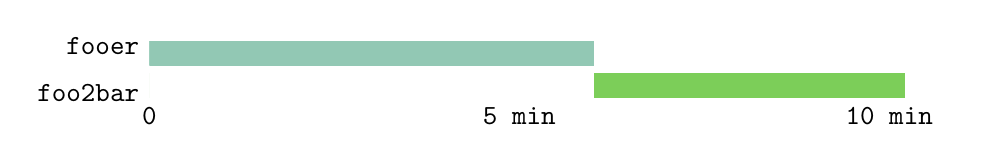
\begin{tikzpicture}
\begin{axis}[
    xbar, xmin=0,
    y axis line style = { opacity = 0 },
    tickwidth         = 0pt,
    width=\textwidth,
    symbolic y coords={fooer,foo2bar},
    ytick=data,
    bar shift=0pt,
    y=0.6cm,
    bar width=0.5cm,
    y dir=reverse,
    xtick={1, 500000, 1000000},
    xticklabels={0, 5 min, 10 min},
    scaled x ticks=false
]


\addplot+[color1, forget plot]    coordinates { (600000,fooer) };

\addplot+[color2, forget plot]    coordinates { (1020000,foo2bar) };
\addplot+[white, forget plot] coordinates { (600000,foo2bar) };
\addplot [white, forget plot] coordinates { (600000,foo2bar) };

\end{axis}
\end{tikzpicture}





% Times
% 1530175200000 2018-06-28 8:40:00.000000000
% 1530175800000 2018-06-28 8:50:00.000000000
% 1530176220000 2018-06-28 8:50:00.000000000
%
% 0
% 600000
% 1020000
\section*{Tasks}
    \lstset{ breaklines=true,
             postbreak=\mbox{\textcolor{red}{$\hookrightarrow$}\space},
             aboveskip=-8pt,belowskip=-12pt}

    \begin{tcolorbox}[ title=fooer, 
                       colbacktitle=color1, 
                       colback=color1!50!white,
                       coltitle=black ]
        \small
        \begin{tabular}{rp{0.72\linewidth}}
ID: & y23kkipm4p4y7kgdzuc1 \\
Process: & fooer \\
Command: & \begin{lstlisting}
echo foo > fooer.foo.txt
\end{lstlisting} \\
Parameters:& \\
Tags: & \\
Start time:  & 2018-06-28 8:40:00.000000000 +0200 CEST \\
Finish time: & 2018-06-28 8:50:00.000000000 +0200 CEST \\
Execution time: & 7 ms \\
Upstreams: & \\
        \end{tabular}
    \end{tcolorbox}

    \begin{tcolorbox}[ title=foo2bar, 
                       colbacktitle=color2, 
                       colback=color2!50!white, 
                       coltitle=black ]
        \small
        \begin{tabular}{rp{0.72\linewidth}}
ID: & omlcgx0izet4bprr7e5f \\
Process: & foo2bar \\
Command: & \begin{lstlisting}
sed 's/foo/bar/g' ../fooer.foo.txt > fooer.foo.txt.foo2bar.bar.txt
\end{lstlisting} \\
Parameters:& \\
Tags: & \\
Start time: & 2018-06-28 8:50:00.000000000 +0200 CEST \\
Finish time: & 2018-06-28 8:50:00.000000000 +0200 CEST \\
Execution time: & 6 ms \\
Upstreams: & \\
        \end{tabular}
    \end{tcolorbox}

\end{document}
